\documentclass[tikz, margin=1mm]{standalone}

\usepackage{cmbright}
\usepackage{xcolor}
% Define colors (personal preferences)
\definecolor{myblack}{HTML}{3B4252}
\definecolor{myblue}{HTML}{1982C4}
\definecolor{myred}{HTML}{FF5C61}
\definecolor{mydarkgray}{HTML}{4C566A}
\definecolor{mybrown}{HTML}{997B66}
\definecolor{mypaleorange}{HTML}{F1DCA7}

\begin{document}

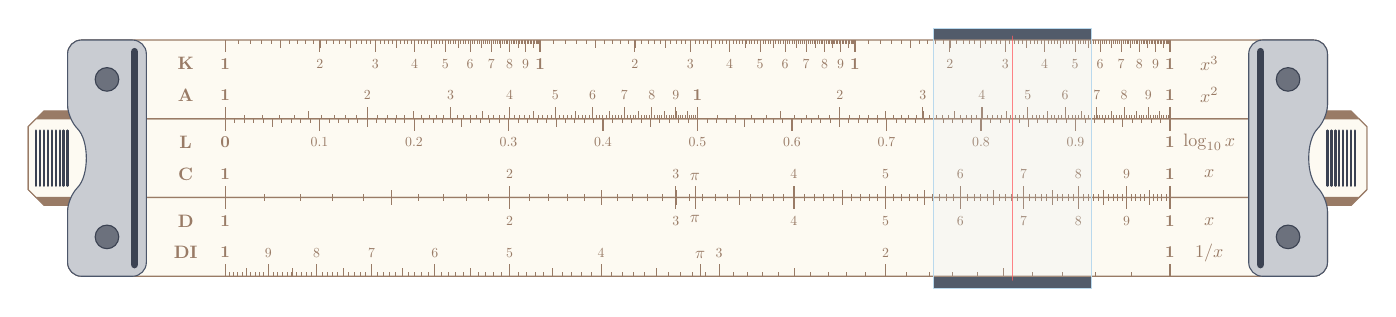
\begin{tikzpicture}

% CURSOR (BACK)
\fill[myblack, line join=round] (9,-1.15) rectangle (11,2.15);

% SLIDE
\begin{scope}
\draw[mybrown, fill=mybrown, line join=round] (-2.3,-0.1) -- (-2.5,0.1) -- (-2.5,0.9) -- (-2.3,1.1) -- (14.3,1.1) -- (14.5,0.9) -- (14.5,0.1) -- (14.3,-0.1) -- cycle;
\draw[mybrown, fill=mypaleorange!15, line join=round] (-2.4,0) -- (-2.5,0.1) -- (-2.5,0.9) -- (-2.4,1) -- (14.4,1) -- (14.5,0.9) -- (14.5,0.1) -- (14.4,0) -- cycle;
\foreach \i in {-2.4,-2.35,...,-2.0} {
  \draw [myblack, line cap=round, line width=0.30mm] (\i,0.15) -- (\i,0.85);
}
\foreach \i in {14,14.05,...,14.4} {
  \draw [myblack, line cap=round, line width=0.30mm] (\i,0.15) -- (\i,0.85);
}

%%% L SCALE
\foreach \i in {0,1,...,9} {
  \foreach \j in {0,1,...,10} {
    \draw[mybrown, very thin] ({1.2*(\i+\j/10},1) -- ++(0,-0.05);
  }
  \foreach \j in {0,5,10} {
    \draw[mybrown, very thin] ({1.2*(\i+\j/10},1) -- ++(0,-0.10);
  }
}
\foreach \i in {0,0.1,0.2,0.3,0.4,0.5,0.6,0.7,0.8,0.9,1} {
  \draw[mybrown] ({12*\i},1) -- ++(0,-0.15);
}
\foreach \i in {0.1,0.2,0.3,0.4,0.5,0.6,0.7,0.8,0.9} {
  \node[mybrown, scale=0.5] at ({12*\i}, 0.7) {\i};
}
\foreach \i in {0,1} {
  \node[mybrown, scale=0.6] at ({12*\i}, 0.7) {\bfseries \i};
}
\node[mybrown, scale=0.65] at (-0.5,0.7) {\bfseries L};
\node[mybrown, scale=0.65] at (12.5,0.7) {$\log_{10}x$};

%%% C SCALE
\foreach \j in {1,1.1,...,10} {
  \draw[mybrown, very thin] ({12*log10(\j)},0) -- ++(0,0.05);
}
\foreach \j in {1,1.5,...,10} {
  \draw[mybrown, very thin] ({12*log10(\j)},0) -- ++(0,0.1);
}
\foreach \j in {1,2,...,9} {
  \draw[mybrown] ({12*log10(\j)},0) -- ++(0,0.15);
}
\foreach \j in {2,...,9} {
  \node[mybrown, scale=0.5] at ({12*log10(\j)}, 0.3) {\j};
}
\foreach \i in {0,1} {
  \node[mybrown, scale=0.6] at ({12*(\i)}, 0.3) {\bfseries 1};
}
\draw[mybrown, very thin] ({12*log10(pi)},0) -- ++(0,0.15) node [above, scale=0.6] {$\pi$};
\node[mybrown, scale=0.65] at (-0.5,0.3) {\bfseries C};
\node[mybrown, scale=0.65] at (12.5,0.3) {$x$};
\end{scope}

% UPPER STATOR
\begin{scope}
\draw[mybrown, fill=mypaleorange!15, rounded corners=5pt] (-2,1) rectangle (14,2);

%%% K SCALE
\foreach \i in {0,1,2} {
  \foreach \j in {1,1.1,...,10} {
    \draw[mybrown, very thin] ({4*(\i+log10(\j)},2) -- ++(0,-0.05);
  }
  \foreach \j in {1,1.5,...,10} {
    \draw[mybrown, very thin] ({4*(\i+log10(\j)},2) -- ++(0,-0.1);
  }
  \foreach \j in {1,2,...,9} {
    \draw[mybrown] ({4*(\i+log10(\j)},2) -- ++(0,-0.15);
  }
  \foreach \j in {2,...,9} {
    \node[mybrown, scale=0.5] at ({4*(\i+log10(\j))}, 1.7) {\j};
  }
}
\foreach \i in {0,1,2,3} {
  \node[mybrown, scale=0.6] at ({4*(\i)}, 1.7) {\bfseries 1};
}
\node[mybrown, scale=0.65] at (-0.5,1.7) {\bfseries K};
\node[mybrown, scale=0.65] at (12.5,1.7) {$x^3$};

%%% A SCALE
\foreach \i in {0,1} {
  \foreach \j in {1,1.1,...,10} {
    \draw[mybrown, very thin] ({6*(\i+log10(\j)},1) -- ++(0,0.05);
  }
  \foreach \j in {1,1.5,...,10} {
    \draw[mybrown, very thin] ({6*(\i+log10(\j)},1) -- ++(0,0.1);
  }
  \foreach \j in {1,2,...,9} {
    \draw[mybrown] ({6*(\i+log10(\j)},1) -- ++(0,0.15);
  }
  \foreach \j in {2,...,9} {
    \node[mybrown, scale=0.5] at ({6*(\i+log10(\j))}, 1.3) {\j};
  }
}
\foreach \i in {0,1,2} {
  \node[mybrown, scale=0.6] at ({6*(\i)}, 1.3) {\bfseries 1};
}
\node[mybrown, scale=0.65] at (-0.5,1.3) {\bfseries A};
\node[mybrown, scale=0.65] at (12.5,1.3) {$x^2$};
\end{scope}

% LOWER STATOR
\begin{scope}
\draw[mybrown, fill=mypaleorange!15, rounded corners=5pt] (-2,-1) rectangle (14,0);

%%% D SCALE
\foreach \j in {1,1.1,...,10} {
  \draw[mybrown, very thin] ({12*log10(\j)},0) -- ++(0,-0.05);
}
\foreach \j in {1,1.5,...,10} {
  \draw[mybrown, very thin] ({12*log10(\j)},0) -- ++(0,-0.1);
}
\foreach \j in {1,2,...,9} {
  \draw[mybrown] ({12*log10(\j)},0) -- ++(0,-0.15);
}
\foreach \j in {2,...,9} {
  \node[mybrown, scale=0.5] at ({12*log10(\j))}, -0.3) {\j};
}
\foreach \i in {0,1} {
  \node[mybrown, scale=0.6] at ({12*(\i)}, -0.3) {\bfseries 1};
}
\draw[mybrown, very thin] ({12*log10(pi)},0) -- ++(0,-0.15) node [below, scale=0.6] {$\pi$};
\node[mybrown, scale=0.65] at (-0.5,-0.3) {\bfseries D};
\node[mybrown, scale=0.65] at (12.5,-0.3) {$x$};

%%% Escala DI
\foreach \i in {0} {
  \foreach \j in {1,1.1,...,10} {
    \draw[mybrown, very thin] ({12*(1-\i-log10(\j)},-1) -- ++(0,0.05);
  }
}
\foreach \i in {0} {
  \foreach \j in {1,1.5,...,10} {
    \draw[mybrown, very thin] ({12*(1-\i-log10(\j)},-1) -- ++(0,0.1);
  }
}
\foreach \i in {0} {
  \foreach \j in {1,2,...,9} {
    \draw[mybrown] ({12*(1-\i-log10(\j)},-1) -- ++(0,0.15);
  }
}
\foreach \i in {0} {
  \foreach \j in {2,...,9} {
    \node[mybrown, scale=0.5] at ({12*(1-\i-log10(\j))}, -0.7) {\j};
  }
}
\foreach \i in {0,1} {
  \node[mybrown, scale=0.6] at ({12*(1-\i)}, -0.7) {\bfseries 1};
}
\draw[mybrown, very thin] ({12*(1-log10(pi))},-1) -- ++(0,0.15) node [above, scale=0.6] {$\pi$};
\node[mybrown, scale=0.65] at (-0.5,-0.7) {\bfseries DI};
\node[mybrown, scale=0.65] at (12.5,-0.7) {$1/x$};
\end{scope}

\foreach \i in {0,12} {
 \foreach \j in {-1,0,1} {
   \draw[mybrown] (\i,\j) -- ++(0,0.15);
   \draw[mybrown] (\i,{\j+1}) -- ++(0,-0.15);
 }
}

% BRACE (POST)
\draw[mydarkgray, fill=mydarkgray!30, rounded corners=5pt] (-2,2) -- (-2,1) to[out=-45, in=45] (-2,0) -- (-2,-1) -- (-1,-1) -- (-1,2) -- cycle;
\draw[mydarkgray, fill=mydarkgray!30, rounded corners=5pt] (14,2) -- (14,1) to[out=225, in=135] (14,0) -- (14,-1) -- (13,-1) -- (13,2) -- cycle;
\draw[myblack, line cap=round, line width=1mm] (-1.15,-0.85) -- (-1.15,1.85);
\draw[myblack, line cap=round, line width=1mm] (13.15,-0.85) -- (13.15,1.85);
\foreach \i in {-1.5,13.5} {
  \foreach \j in {-0.5,1.5} {
    \draw[myblack, fill=myblack!75] (\i,\j) circle [radius=0.15];
  }
}

% CURSOR (FRONT)
\draw[myblue!30, fill=myblue!15, line join=round, fill opacity=0.15] (9,-1.15) rectangle (11,2.15);
\draw[myred, line cap=round, opacity=0.75] (10,-1.05) -- (10,2.05);

\end{tikzpicture}

\end{document}